% VanniKawachh -- IEEE conference paper (v2 concept)
% Source: docs/RESEARCH_PAPER.md. All measured numbers (68/68 unit cases,
% 8/8 SITL acceptance, 0.4-0.6 m terminal accuracy, Phase-0 rehearsal with
% fused severity 0.88 and kit release at 3.1 m, 328 s mission) are shared
% with the journal version; neither document may claim acoustic accuracy
% figures or hardware radio/range measurements (Phase 1-2 work in progress).
\documentclass[conference]{IEEEtran}

\usepackage{amsmath}
\usepackage{amssymb}
\usepackage{graphicx}
\usepackage{booktabs}
\usepackage{url}
\usepackage{cite}

\graphicspath{{../figures/v2/}{../figures/}}

\begin{document}

\title{VanniKawachh: A Distributed AI Acoustic Intelligence and
Autonomous Drone Response Network for Women Safety}

\author{
\IEEEauthorblockN{Shivansh Verma, Saksham Sabadra, Rudra Thakur, and Rohan Untawale}
\IEEEauthorblockA{Group CSE\_B\_04, Department of Computer Science and Engineering\\
G. H. Raisoni College of Engineering, Nagpur, India\\
Guide: Dr. Aditya Turankar\\
Repository: \url{https://github.com/SV-1411/drone.git}}
}

\maketitle

\begin{abstract}
Crimes against women often happen in surveillance and cellular dead
zones such as dark streets, forest stretches, and campus outskirts.
Most safety technology puts the burden on the victim: panic apps,
wearables, and carried devices only work while a charged, reachable
device is in the victim's hand. We present \emph{VanniKawachh}, a
three-tier network that moves the trigger burden from the victim to
the infrastructure. Her voice is the trigger. Solar-powered,
pole-mounted sensing nodes (ESP32-S3 + INMP441) screen every audio
frame on-device with a lightweight MFCC + CNN model (Stage~1,
$<$50~ms budget, recall-tuned), so no continuous audio ever leaves a
pole. A Raspberry Pi~5 hub confirms candidate events with PANNs deep
audio tagging fused with PIR motion, ambient-light, and time-of-day
evidence (Stage~2, precision-tuned), and dispatches only above
explicit verification and severity thresholds. A confirmed alert is a
25-byte packet sealed with AES-128-CTR, a truncated HMAC-SHA256 tag,
and a per-node replay counter. It carries surveyed node coordinates
from a registry rather than a live GPS fix, and travels over LoRa
with no cellular dependency to a police dashboard. The same alert
auto-dispatches an autonomous quadcopter that records evidence during
hover, descends to 3~m, drops a first-aid kit (on failure it returns
to launch), and returns. The response layer is our previously
SITL-verified flight stack (verified mode transition, a
landing-interlocked mission queue, and a debounced severity-ordered
failsafe arbiter), carried over unchanged. The complete chain runs
end-to-end with zero hardware: the Phase-0 rehearsal passed with
fused severity 0.88 and kit release commanded at 3.1~m inside a 328~s
SITL mission; the acceptance harness passes 8/8 checks with 0.4 to
0.6~m terminal accuracy; 68 automated unit cases cover the safety
logic, packet cryptography, and dispatch gating. Stage-1 model
training and hardware range measurements are Phase 1 and 2 work in
progress. The development chain used clearly labelled heuristic
stand-ins, and this paper reports no acoustic accuracy it has not
measured.
\end{abstract}

\begin{IEEEkeywords}
women safety; acoustic event detection; TinyML; PANNs; sensor fusion;
LoRa; AES-128; autonomous UAV; verified dispatch; SITL.
\end{IEEEkeywords}

\section{Introduction}
\label{sec:intro}

Safety technology fails where assaults happen: in places with few
cameras, few patrols, and often no cellular coverage, at moments when
the victim cannot operate a device because her hands are occupied or
the phone is snatched, discharged, or out of reach. The deployed
answer to women's safety has been to instrument the victim with panic
buttons, mobile apps, and smart wearables. The best of these report
high trigger accuracy, but their failure mode is structural: a
device-borne trigger protects only the moments in which the device is
present, charged, and reachable.

VanniKawachh (``voice-shield'') moves the burden. Pole-mounted
infrastructure listens. A scream, a cry, or a shouted ``help'' /
``bachao'' is the trigger, and the victim needs no device to produce
it. The engineering problem then has three parts: (i)~detection must
run on a solar pole budget without streaming audio anywhere;
(ii)~false alarms must be suppressed well enough that acting on an
alert is defensible, because the action is a drone launch; and
(iii)~the alert path must work exactly where cellular does not, and
it must be unforgeable, because a spoofed alert would launch the
drone for an attacker.

Our contributions are:
\begin{enumerate}
\item An \textbf{end-to-end architecture} covering infrastructure
  sensing, two-stage verification, offline encrypted alerting, and
  autonomous field response, where surveyed prior work covers at most
  one link (Section~\ref{sec:related}).
\item A \textbf{two-stage acoustic pipeline} that splits recall and
  precision between an on-node TinyML screen and a hub-side PANNs +
  sensor-fusion confirmation, with tested dispatch gating
  (Section~\ref{sec:pipeline}).
\item A \textbf{secure LoRa alert protocol}: sealed 25-byte packets
  resolved against a surveyed node registry, so position is never
  transmitted or trusted from the field (Section~\ref{sec:lora}).
\item A \textbf{safety-verified autonomous response layer}: our
  SITL-verified dispatch stack, extended with an evidence camera
  window and a rule-bounded first-aid kit drop
  (Section~\ref{sec:response}).
\item A \textbf{zero-hardware full-chain validation} (Phase~0) that
  runs the integrated system in software-in-the-loop simulation and
  states which numbers are measured and which await the hardware
  phases (Section~\ref{sec:eval}).
\end{enumerate}

\section{Related Work}
\label{sec:related}

Our twelve-paper survey (2023 to 2026; entries [S1] to [S12], full
bibliography in the group's seminar record and the journal
version)~\cite{survey} splits the field on one question: who carries
the trigger?

\textbf{Victim-carried devices} (survey entries [S1], [S5], [S6],
[S9], [S10], [S11] of~\cite{survey}) include apps, wearables, and IoT
panic buttons. They report trigger-classification accuracies up to
\textbf{97.5\%}, typically with GPS + GSM alerting. All of them fail
the same way when the device is absent, damaged, discharged, or
unreachable, and they depend on cellular coverage in exactly the
locations that lack it.

\textbf{Detection-only audio systems} (entries [S2], [S3], [S4], [S7],
[S8] of~\cite{survey}) reach \textbf{92 to 95.5\%} scream detection
with CNN-Transformer hybrids and transfer-learned backbones
(InceptionV3, MobileNetV2) on mel-spectrograms. But they run on
server-scale compute, are evaluated on curated data, and stop at
classification: no location delivery, no dead-zone alerting, no
response.

\textbf{The gap} is the chain itself. No surveyed system provides
infrastructure sensing, verified offline alerting, and autonomous
response end to end. Each link is supported by adjacent work:
TensorFlow Lite Micro keyword spotting~\cite{tflm} for the node,
PANNs large-scale pretrained audio tagging~\cite{panns} for the hub,
LPWAN practice~\cite{sx1278} for the alert path, and the open-source
autopilot ecosystem~\cite{ardupilot,mavlink} for the response. Our
prior flight-stack work supplies the response layer's safety
machinery, including the finding that shaped the design philosophy:
flight autopilots can \emph{silently reject} mode commands while
client libraries report success. VanniKawachh applies the resulting
rule, \emph{a claim is not a confirmation}, to every layer: sound,
packet, dispatch, and flight mode.

\section{System Architecture}
\label{sec:arch}

\begin{figure}[!t]
\centering
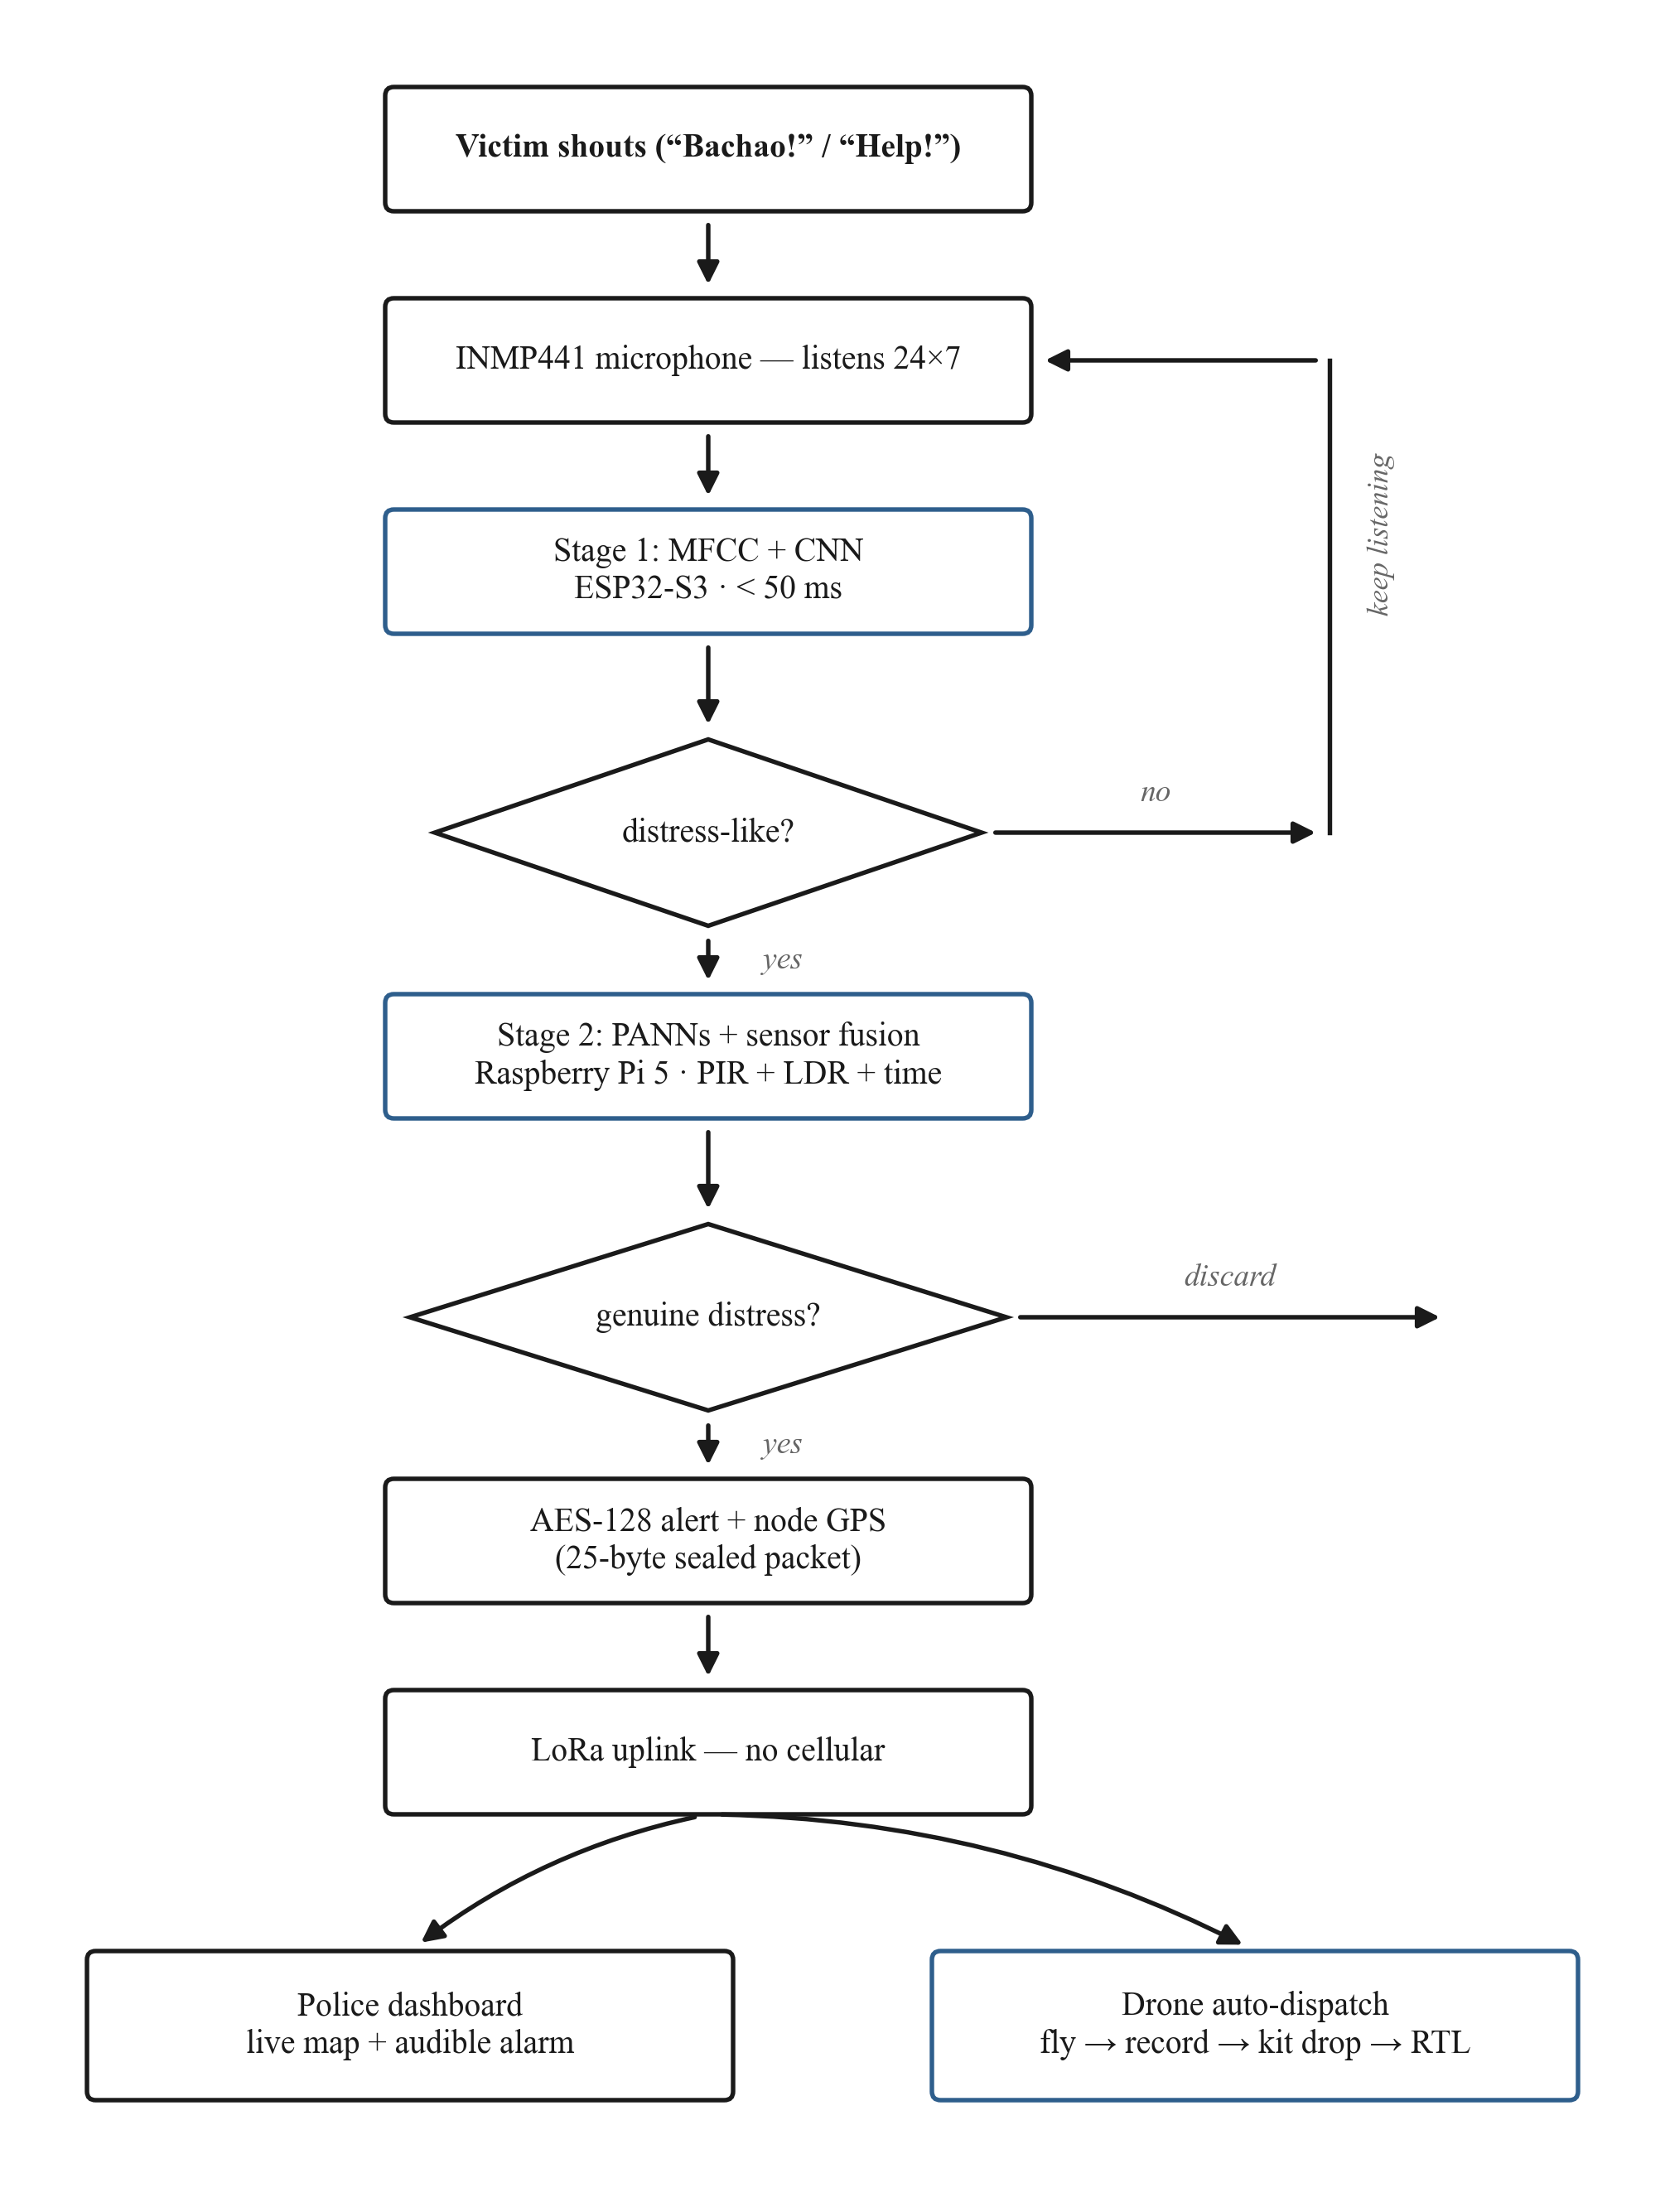
\includegraphics[width=\columnwidth]{fig2_methodology.png}
\caption{The VanniKawachh chain, from acoustic event through Stage-1
on-node screening, Stage-2 hub verification and fusion, and sealed
LoRa alerting to the parallel dashboard and drone-dispatch paths. Each
tier verifies before it acts.}
\label{fig:methodology}
\end{figure}

Fig.~\ref{fig:methodology} traces one incident through the three
tiers: the solar-powered sensing node (ESP32-S3 + INMP441, PIR + LDR
context, Stage-1 hit $\rightarrow$ sealed alert over LoRa + 4~s clip
over ESP-NOW/WiFi), the Raspberry Pi~5 hub (unseal, registry lookup,
Stage-2 PANNs + fusion, police dashboard, \texttt{POST /trigger}), and
the SITL-verified response drone (trigger API $\rightarrow$ queue
$\rightarrow$ 13-state FSM with hover-record, 3~m kit drop, and RTL).

Three design decisions shape the architecture. \textbf{Fixed nodes
carry no live GPS.} Each pole is surveyed once at installation. The
hub's registry maps \texttt{node\_id} $\rightarrow$ (lat, lon), so the
radio carries two bytes of identity, and a node has no GPS to spoof,
jam, or drain. \textbf{LoRa carries the alert, never the audio.}
LoRa's effective throughput of about 1 to 5.5~kbps cannot move a clip,
so the sealed alert goes over LoRa at once while the 4~s verification
clip follows over ESP-NOW/WiFi (about 250~kbps, hundreds of metres
line of sight). If the clip does not arrive within 8~s, the hub falls
back to the Stage-1 confidence scaled by 0.6; it always logs the
incident, and dispatches only if the remaining evidence is strong.
\textbf{The flight core is untouched.} All v1 safety machinery carries
over unchanged, which is why the response half of the system already
works.

\section{The Two-Stage Acoustic Pipeline}
\label{sec:pipeline}

\textbf{Stage 1 (node, recall-tuned).} The ESP32-S3 frames 16~kHz mono
audio from the INMP441, extracts MFCCs, and runs a tiny quantized CNN
(TensorFlow Lite Micro, \texttt{micro\_speech}-class~\cite{tflm})
against the distress vocabulary (scream, cry, and the
``help''/``bachao'' keywords) within a $<$50~ms per-frame budget. The
front end is the standard speech chain: each frame is pre-emphasised,
\begin{equation}
\label{eq:preemph}
y[n] = x[n] - 0.97\,x[n-1],
\end{equation}
Hamming-windowed,
\begin{equation}
\label{eq:hamming}
w[n] = 0.54 - 0.46\cos\!\left(\frac{2\pi n}{N-1}\right),
\end{equation}
and its magnitude spectrum pooled by $M$ triangular filters spaced
uniformly on the mel scale
\begin{equation}
\label{eq:mel}
m = 2595\,\log_{10}\!\left(1 + \frac{f}{700}\right),
\end{equation}
giving log filterbank energies
\begin{equation}
\label{eq:fbank}
e_j = \log \sum_{k} \lvert X(k)\rvert^2\, H_j(k),
\end{equation}
which a DCT-II decorrelates into the 13 cepstral coefficients used as
the per-frame feature vector,
\begin{equation}
\label{eq:dct}
c_i = \sum_{j=1}^{M} e_j
\cos\!\left[\, i\left(j - \tfrac{1}{2}\right)\frac{\pi}{M}\right],
\qquad i = 1,\dots,13.
\end{equation}
The CNN classifies each MFCC frame through a softmax output,
\begin{equation}
\label{eq:softmax}
p_i = \frac{\exp(z_i)}{\sum_j \exp(z_j)},
\end{equation}
is trained with the cross-entropy loss
\begin{equation}
\label{eq:xent}
L = -\sum_i y_i \log p_i,
\end{equation}
and deploys after int8 post-training quantization,
\begin{equation}
\label{eq:quant}
x_q = \mathrm{round}\!\left(\frac{x}{s}\right) + z,
\end{equation}
with per-tensor scale $s$ and zero-point $z$. This quantization step
fits the model into TFLM on the ESP32-S3. Frames that do not trip
Stage~1 are discarded on the spot: nothing is stored and nothing is
transmitted. Stage~1 exists to avoid misses; its false positives are
expected and cheap because Stage~2 filters them. (The model itself is
a hook in the current firmware; training and flashing it is Phase-1
work, see Section~\ref{sec:measured}.)

\textbf{Stage 2 (hub, precision-tuned).} The hub re-scores the clip
with PANNs~\cite{panns}, the pretrained AudioSet tagging network
(CNN14, or a lighter checkpoint on a slow Pi). It takes the summed
probability over the distress-relevant AudioSet classes (screaming,
shouting, yelling, crying, wailing, and similar) as a distress score
in $[0, 1]$. No bespoke training is required; the hub relies on
AudioSet scale, which a locality Pi~5 can afford and a solar pole
cannot. A labelled energy-heuristic fallback backend (loud, high
spectral centroid, bursty) exists so the whole chain runs on any
development machine. It is not a claim of accuracy, and every result
produced with it is marked as fallback.

\textbf{Fusion.} A night-time scream in a dark spot with motion nearby
carries more weight than a daytime shout on a busy road. With $a$
the Stage-2 audio score, $c$ the Stage-1 confidence, $p \in \{0,1\}$
the PIR motion flag, $d = 1 - L/255$ the darkness derived from the LDR
level $L \in [0,255]$, and $n \in \{0,1\}$ the night indicator (1
during 20:00 to 06:00), the fused severity is
\begin{equation}
\label{eq:fusion}
S = 0.60\,a + 0.15\,c + 0.10\,p + 0.08\,d + 0.07\,n,
\end{equation}
with priority \texttt{high} at $S \geq 0.75$ or verified audio
($a \geq 0.6$) together with PIR motion ($p = 1$). Dispatch requires
\textbf{both} gates to pass,
\begin{equation}
\label{eq:gate}
\mathrm{dispatch} \iff (a \geq \tau_v) \wedge (S \geq \tau_d),
\quad \tau_v = 0.50,\ \tau_d = 0.60;
\end{equation}
below either threshold the incident is logged with a human-readable
reasons trace and no drone flies. When the verification clip never
arrives (Section~\ref{sec:arch}), the degraded audio score
\begin{equation}
\label{eq:degraded}
a = 0.6\,c
\end{equation}
is substituted before applying \eqref{eq:fusion} and \eqref{eq:gate}.
The gating is covered by automated tests, and the weights in
\eqref{eq:fusion} are prototype values to be tuned against Phase-1
bench data.

\section{Secure LoRa Alerting}
\label{sec:lora}

A spoofed packet would launch a drone; a replayed one would launch it
at a time the attacker chooses. Every alert is therefore a sealed
25-byte packet that fits in one LoRa frame, laid out as shown in
Fig.~\ref{fig:packet}: a cleartext header (magic, version,
\texttt{node\_id} uint16, counter uint32), an 8-byte
AES-128-CTR-encrypted payload (event class, Stage-1 confidence, PIR
flag, LDR level, node battery), and an 8-byte MAC (HMAC-SHA256 over
header + ciphertext, truncated).

\begin{figure}[!t]
\centering
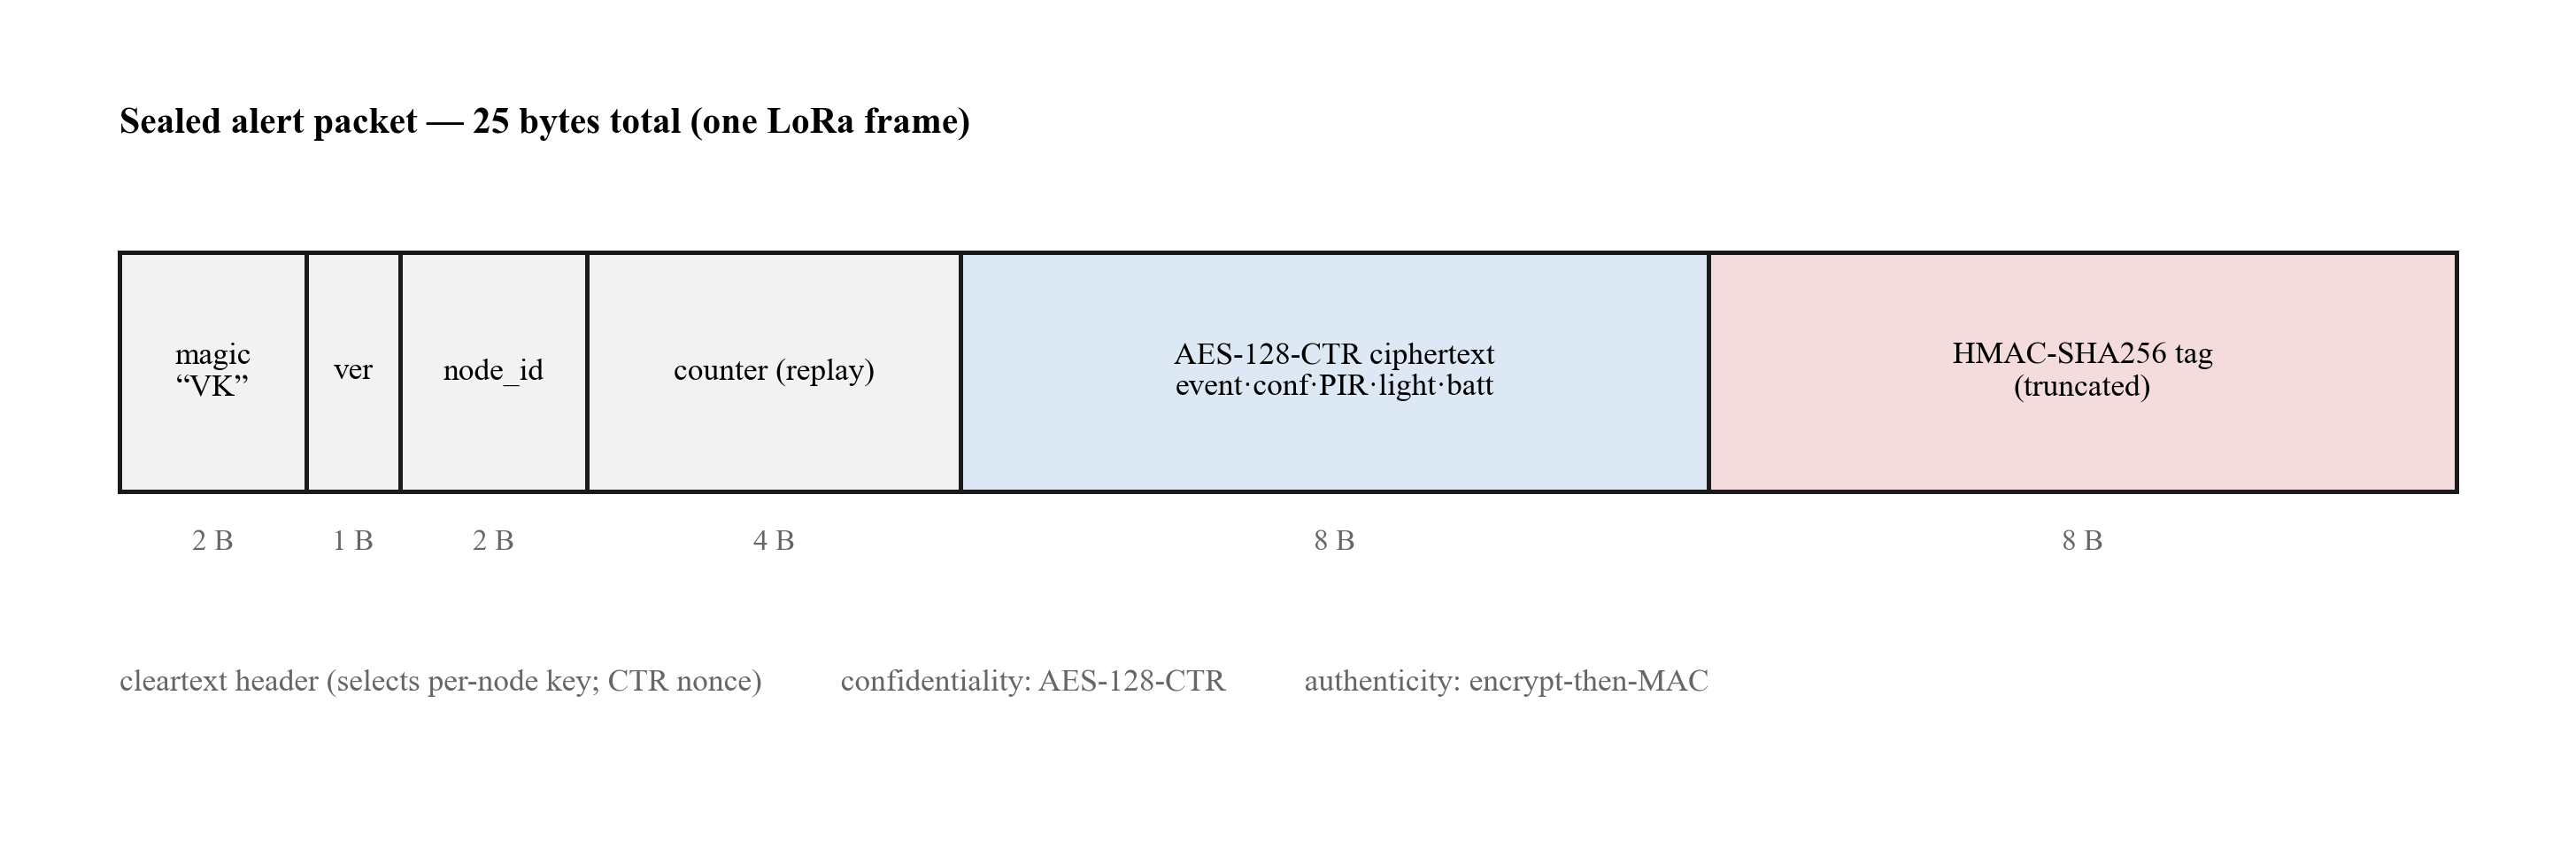
\includegraphics[width=\columnwidth]{fig4_packet.png}
\caption{The 25-byte sealed alert packet: cleartext header,
AES-128-CTR ciphertext, and truncated HMAC-SHA256 tag, all in one
LoRa frame.}
\label{fig:packet}
\end{figure}

Per-node keys derive from the master key $K_m$ by keyed hashing
(FIPS-197 AES, RFC 2104 HMAC~\cite{fips197hmac}),
\begin{equation}
\label{eq:keyderive}
K_n = \mathrm{HMAC\mbox{-}SHA256}\!\left(K_m,\ \texttt{"node:"} \,\|\, n\right)[0{:}16],
\end{equation}
so provisioning needs only the master key and an id. A captured node
compromises one pole, and that node can be revoked in the registry.
The payload $P$ is encrypted in CTR mode,
\begin{equation}
\label{eq:ctr}
C = P \oplus E_{K_n}(\mathrm{IV}),
\end{equation}
with the counter block IV built from the cleartext header
(magic $\|$ ver $\|$ node\_id $\|$ counter), which is unique per
packet while the counter is monotonic. Authentication is
encrypt-then-MAC,
\begin{equation}
\label{eq:mac}
\tau = \mathrm{HMAC\mbox{-}SHA256}\!\left(K_n,\ \mathrm{header} \,\|\, C\right)[0{:}8].
\end{equation}
The hub accepts a packet only when
\begin{equation}
\label{eq:accept}
\tau\ \mathrm{valid}\ \wedge\ \mathrm{counter} > \mathrm{counter}_{\mathrm{last}},
\end{equation}
so bad MACs, unknown node ids, and replays are all rejected. Forging
the 64-bit truncated tag succeeds with probability $2^{-64}$ per
attempt. Above the radio, the hub reaches the drone stack through the
same token-authenticated, geofence-validated API as any operator;
there is no privileged backdoor. Residual risk is stated: jamming can
deny service but cannot forge an alert; multi-node corroboration and
node-liveness monitoring are future answers.

The LoRa/WiFi split of Section~\ref{sec:arch} follows from the
physics. LoRa's range comes from spreading. Each symbol lasts
\begin{equation}
\label{eq:symtime}
T_s = \frac{2^{\mathrm{SF}}}{\mathrm{BW}},
\end{equation}
and the receiver sensitivity floor
\begin{equation}
\label{eq:sens}
S_{\mathrm{dBm}} = -174 + 10\log_{10}(\mathrm{BW}) + \mathrm{NF} + \mathrm{SNR}_{\min}
\end{equation}
drops below $-120$~dBm at high SF over $\mathrm{BW} = 125$~kHz, so
milliwatts reach kilometres. The same trade caps throughput: the
standard LoRa time-on-air expression (Semtech SX127x
datasheet~\cite{sx1278}) gives $\approx 0.21$~s for the 25-byte sealed
alert at SF9, BW 125~kHz, CR 4/5, explicit header + CRC, whereas the
4~s clip ($\approx 128$~kB at $\approx 5.5$~kb/s effective) would
occupy the channel for minutes. So the alert goes over LoRa and the
clip over ESP-NOW/WiFi.

Privacy is built into the design: continuous audio cannot leave a
node because the transport cannot carry it and the clip path is
event-gated in firmware. Only event-triggered clips $\leq 5$~s are
ever transmitted, and the alert itself is encrypted.

\section{Safety-Verified Drone Response}
\label{sec:response}

The response layer is our SITL-verified dispatch stack. Its three
mechanisms transfer intact. \textbf{Verified mode transition:} every
flight-mode command, nominal or emergency, routes through a single
routine. The routine re-issues the request through layered MAVLink
encodings (\texttt{COMMAND\_LONG}/\texttt{MAV\_CMD\_DO\_SET\_MODE}
plus the legacy \texttt{SET\_MODE}) every 700~ms until the autopilot's
own HEARTBEAT-derived mode confirms adoption, with a cross-action
fallback (RTL $\rightleftarrows$ LAND) on the abort path. This design
answers the silent rejection we observed on ArduCopter 3.3 SITL.
\textbf{Landing interlock:} every abnormal termination blocks until
the vehicle demonstrably lands and disarms (bounded 240~s) before the
queue regains control, and a dequeued mission refuses to arm an armed
vehicle. Together, these mean the queue can never start a flight
against an airborne vehicle. \textbf{Failsafe arbitration:} battery,
GPS, geofence, and timeout monitors feed a 1~Hz arbiter with monotone
severity (LAND never downgraded), $N$-sample GPS debounce, fire-once
event semantics, and mid-RTL escalation. Geofence radii, arrival
detection against the 5~m waypoint tolerance, and ETA all use the
haversine great-circle distance
\begin{equation}
\label{eq:haversine}
\begin{split}
d &= 2R \arcsin\sqrt{\sin^2\!\frac{\Delta\varphi}{2} +
\cos\varphi_1 \cos\varphi_2 \sin^2\!\frac{\Delta\lambda}{2}},\\
R &= 6371~\mathrm{km}.
\end{split}
\end{equation}

The thirteen-state mission FSM within which these mechanisms run is
shown in Fig.~\ref{fig:fsm}.

\begin{figure}[!t]
\centering
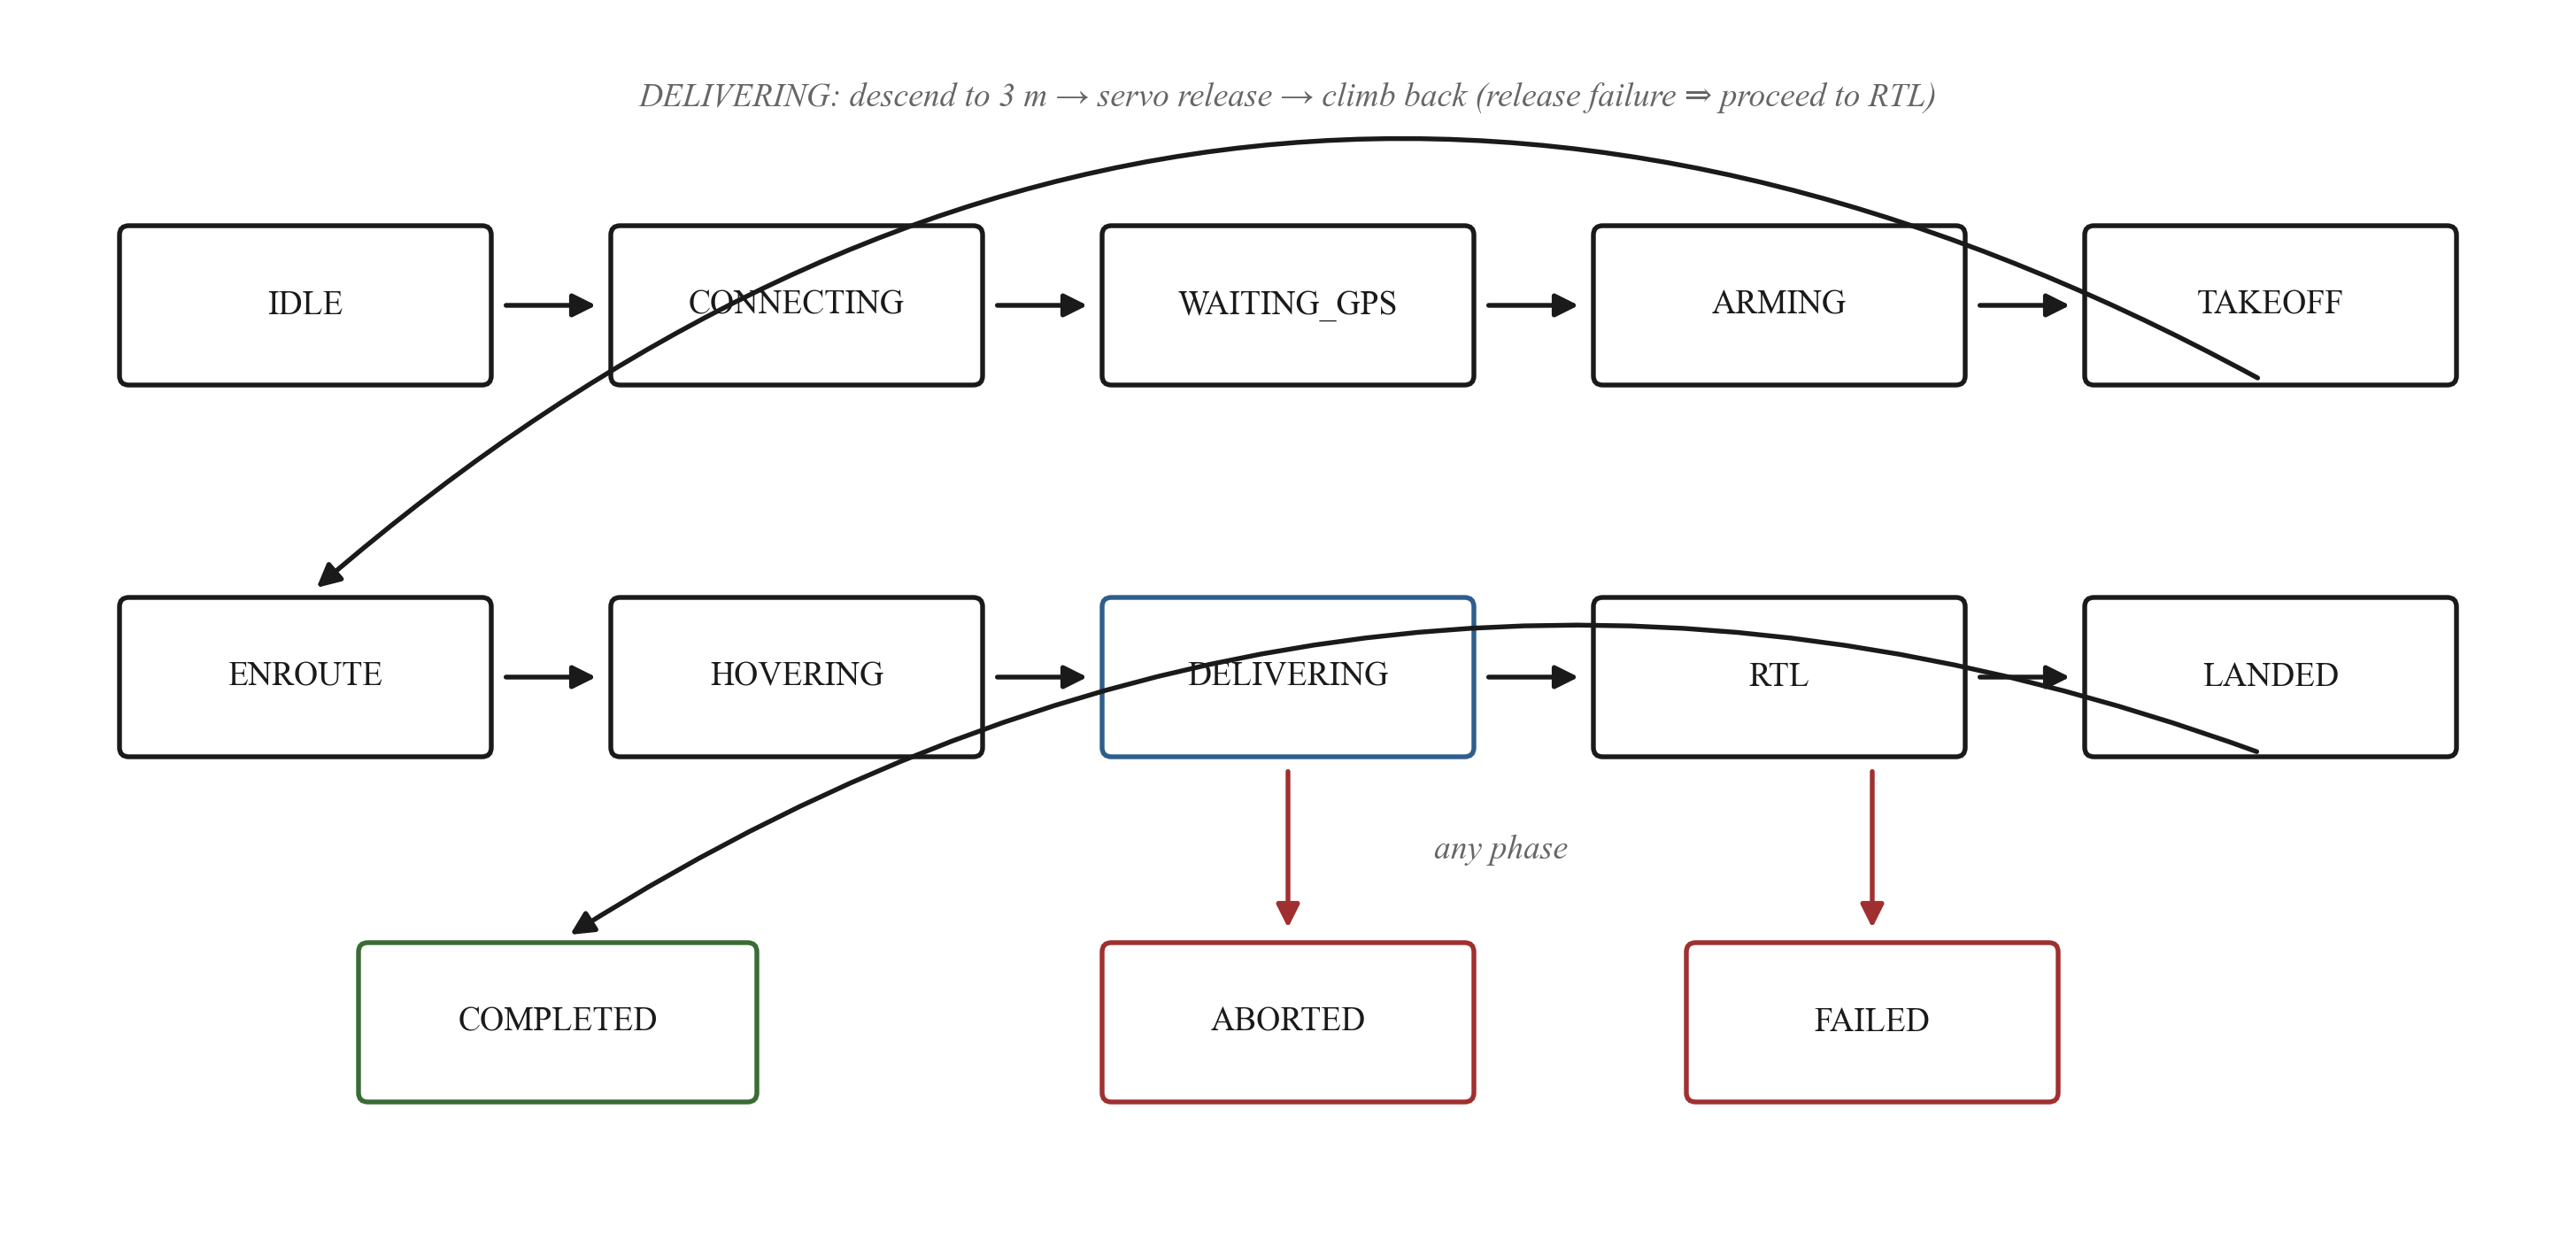
\includegraphics[width=\columnwidth]{fig5_state_machine.png}
\caption{The 13-state mission FSM, from IDLE through TAKEOFF, ENROUTE,
HOVERING, and DELIVERING to RTL and LANDED, with the abnormal paths
into ABORTED and FAILED.}
\label{fig:fsm}
\end{figure}

v2 adds the response payload. The mission FSM (now thirteen states)
records camera evidence during the hover window (Pi Camera Module~3 on
hardware; a no-op stub in SITL, so the flow is byte-identical) and
then enters \textbf{DELIVERING}: descend over the incident point to
the configured drop altitude (3.0~m, tolerance 0.7~m, bounded at
45~s), release the first-aid kit via an SG90 servo on Pixhawk AUX
OUT~1 commanded with \texttt{MAV\_CMD\_DO\_SET\_SERVO} (open 1900 PWM,
2~s settle, re-close 1100), then climb back to cruise altitude for the
RTL. The 3~m rule comes from simple ballistics: a kit released from
height $h$ free-falls for
\begin{equation}
\label{eq:fall}
t = \sqrt{\frac{2h}{g}} \approx 0.78~\mathrm{s}
\quad \text{at } h = 3~\mathrm{m},
\end{equation}
during which a $v_w = 2$~m/s wind drifts it only
\begin{equation}
\label{eq:drift}
x \approx v_w\,t \approx 1.6~\mathrm{m},
\end{equation}
keeping the kit within reach of the victim. A cruise-altitude release
would increase both drift and impact energy. The governing rule is
that \textbf{a failed release is never a reason to loiter}: the
failure is logged and the drone proceeds to RTL regardless. The
DELIVERING loop polls the failsafe arbiter like every other phase, so
a battery or GPS demand pre-empts the drop. All prototype flying is
VLOS-only on a registered airframe with an RC safety pilot, per
India's Drone Rules 2021~\cite{dronerules}; autonomous BVLOS response
is described strictly as a supervised pilot-program pathway.

\section{Evaluation}
\label{sec:eval}

\subsection{Methodology}

Validation is staged. \textbf{Tier 1:} 68 automated unit cases: 47
over the flight stack's safety logic (every arbiter rule, queue
semantics, persistence, every edge-validation bound), 14 over the hub
chain (packet seal/unseal, MAC tamper rejection, replay rejection,
registry, fusion, pipeline gating, where \emph{no dispatch below
threshold} is asserted rather than assumed, and dispatcher payload
shape), and 7 over obstacle keep-out routing. The suites discriminate:
run against the pre-hardening implementation, the debounce, cancel,
and interlock cases fail. \textbf{Tier 2:} an eight-property SITL
acceptance flight (ArduCopter 3.3; 896~m mission at 15~m altitude):
simulator up, API up, connected, armed, took off, reached target
($\leq 5$~m), returned home ($\leq 10$~m, required), landed.
\textbf{Tier 3:} the Phase-0 full-chain rehearsal
(\texttt{scripts/demo\_phase0.py}). A synthesized distress WAV stands
in for the microphone; a simulated node 600~m from home seals a real
packet with the production cryptography; the production hub pipeline
verifies (fallback backend), fuses, gates, and dispatches; and the
production drone stack flies the SITL mission with hover-record and
kit drop. Everything except the audio source, the Stage-2 backend, and
the physics is production code.

\subsection{Results}

Tier 1: \textbf{68/68 pass.} Tier 2: \textbf{8/8 checks pass.} Across
six acceptance missions spanning the development arc, closest approach
was 0.4 to 0.6~m against the 5~m tolerance, and final distance from
home was 0.0 to 0.2~m; terminal accuracy is bounded by the autopilot's
loiter behaviour, not by the dispatch layer. Tier 3: the rehearsal
\textbf{passed end to end}. The sealed alert (event \texttt{scream},
PIR active, dark LDR) was authenticated and replay-checked; the
fallback backend scored the clip above the 0.50 verification
threshold; \textbf{fused severity 0.88} (priority \texttt{high})
cleared the 0.60 dispatch gate; and the SITL mission ran the full
lifecycle with the recording window active and \textbf{kit release
commanded at 3.1~m} relative altitude, completing in \textbf{328~s}
with 0.4~m closest approach. Fig.~\ref{fig:profile} shows the
rehearsal's altitude profile, with the descent to the 3.1~m release
point visible between the hover window and the return leg.

\begin{figure}[!t]
\centering
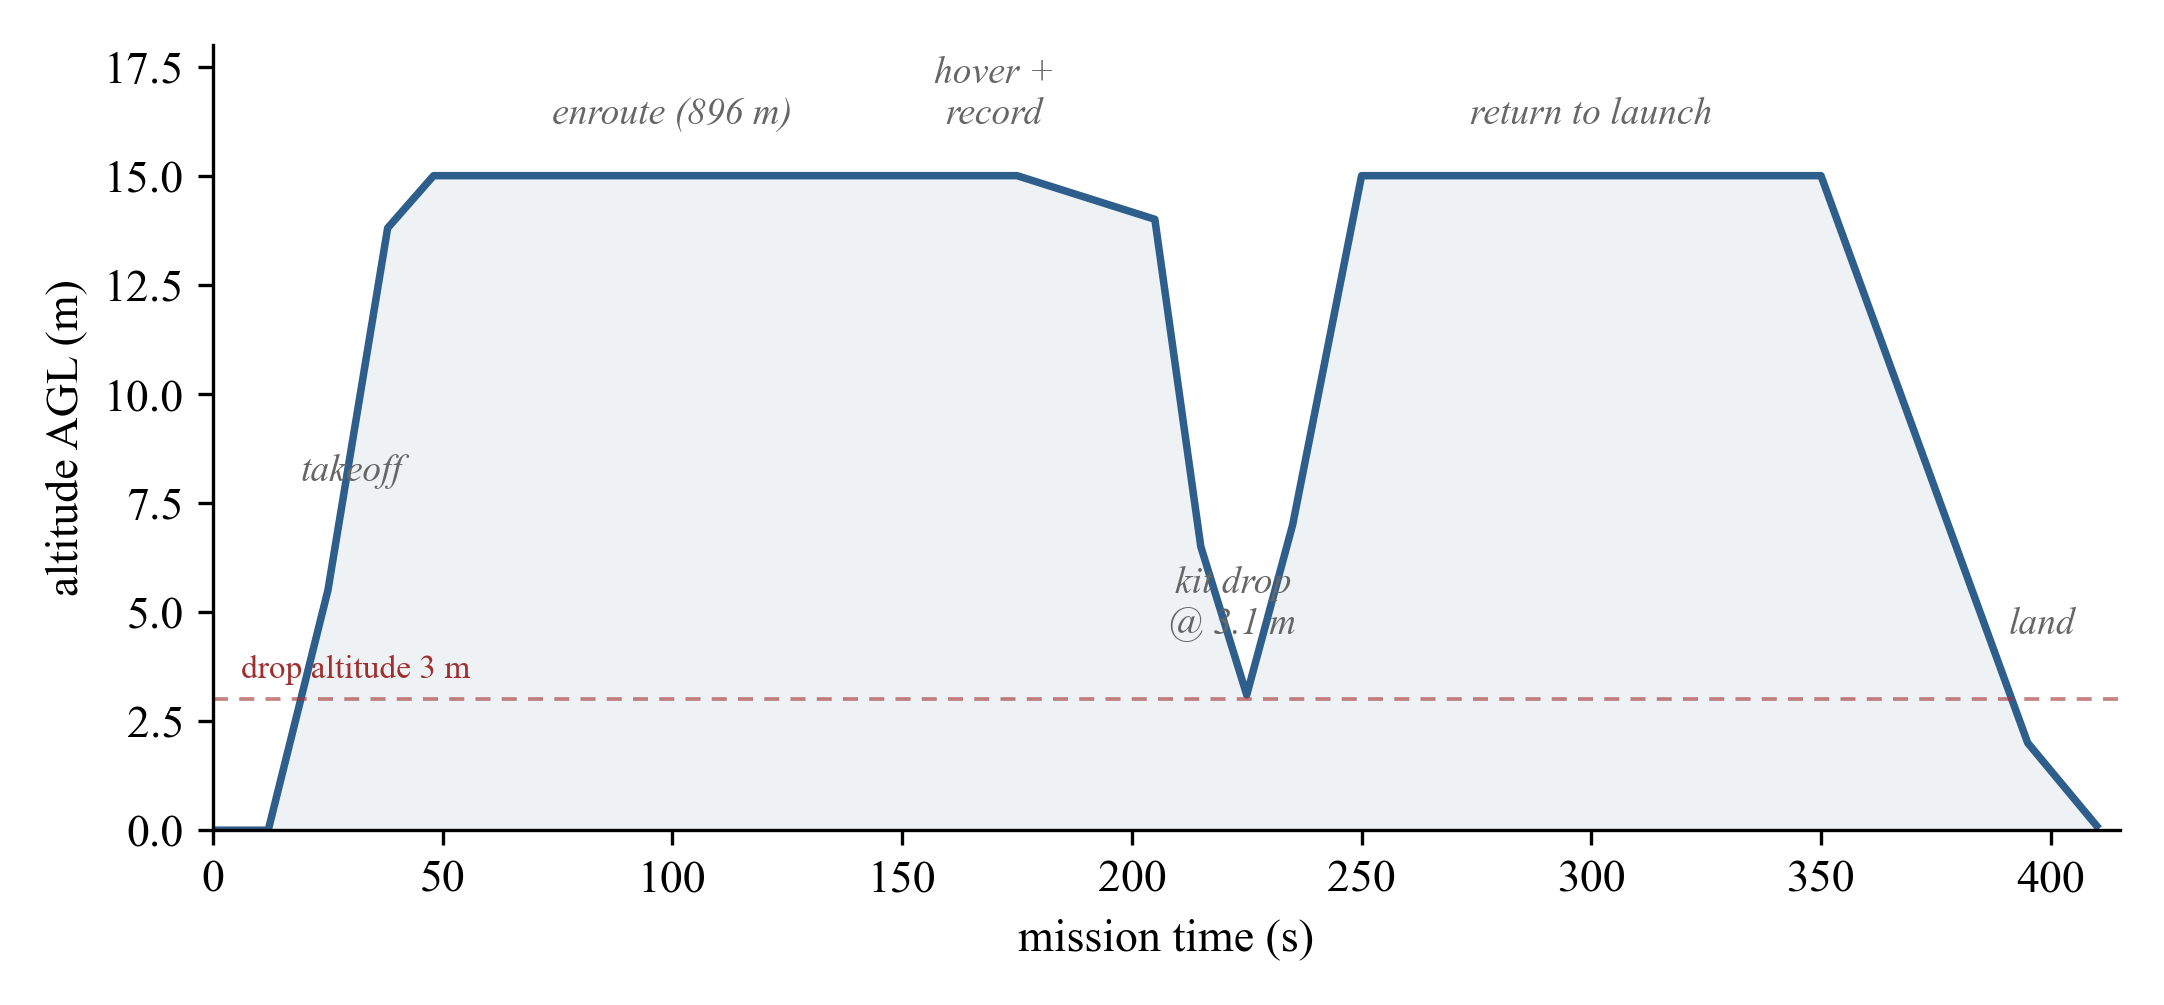
\includegraphics[width=\columnwidth]{fig8_mission_profile.png}
\caption{Altitude profile of the Phase-0 full-chain rehearsal: takeoff
to cruise, transit, hover-observe, descent to the 3.1~m kit release,
climb-out, and return to launch, completing in 328~s.}
\label{fig:profile}
\end{figure}

\subsection{What Is Measured vs.\ In Progress}
\label{sec:measured}

The Phase-0 result proves the architecture and the integration: every
interface a hardware phase will use (packet bytes, clip convention,
thresholds, trigger payload, servo command) was exercised in
production form. It deliberately proves nothing about acoustic
detection performance. \textbf{No Stage-1 accuracy exists.} The TFLM
model is a hook; training and flashing it is Phase~1; $<$50~ms is a
design budget, not a measurement. \textbf{No field Stage-2 accuracy
exists.} The Phase-0 score came from the labelled heuristic fallback
on synthesized audio; PANNs' published performance~\cite{panns}
motivates the backend and is not a field claim. For transparency, the
fallback scorer is fully specified: over the clip samples it computes
the RMS level
\begin{equation}
\label{eq:rms}
\mathrm{RMS} = \sqrt{\frac{1}{N}\sum_{n} x^2[n]},
\end{equation}
the spectral centroid
\begin{equation}
\label{eq:centroid}
C = \frac{\sum_{f} f\,\lvert X(f)\rvert}{\sum_{f} \lvert X(f)\rvert},
\end{equation}
and an envelope-burstiness term, combined as
\begin{equation}
\label{eq:fallback}
\begin{split}
\mathrm{score} = {}& 0.45\,\min\!\left(1, \frac{\mathrm{RMS}}{0.15}\right) \\
& + 0.35\,\mathrm{clip}\!\left(\frac{C - 400}{1600},\,0,\,1\right)
+ 0.20\,\mathrm{burstiness}.
\end{split}
\end{equation}
Equations \eqref{eq:rms} to \eqref{eq:fallback} describe a labelled
development stand-in (loud, high-centroid, bursty audio scores high),
not a detection claim. \textbf{No radio range/loss or ESP-NOW
reliability figures exist} (Phase~2). \textbf{No hardware flight has
occurred.} Phase~3's staged VLOS progression governs the transition;
the SITL firmware is the 2015-vintage 3.3 build, whose
command-delivery faults forced the defensive design. These
measurements (outdoor detection distance vs.\ SNR, per-stage latency,
end-to-end false-positive rate on street noise, LoRa range vs.\
spreading factor) are the explicit deliverables of the Phase 1 and 2
bench campaigns and will appear in the journal version once measured.

\section{Regulatory, Spectrum, and Privacy Grounding}
\label{sec:regulatory}

Deployment legality is part of the design. \textbf{Airspace:} UAS
operation in India is governed by The Drone Rules, 2021
(G.S.R.~589(E), Ministry of Civil Aviation)~\cite{dronerules}, which
require registration on the DGCA's Digital Sky platform and divide
airspace into green, yellow, and red zones. All prototype flying sits
in the least-restrictive cell of that framework: a registered
airframe, VLOS-only, in green-zone private airspace, with an RC safety
pilot holding override authority. Autonomous BVLOS response is framed
strictly as a supervised pilot-program pathway contingent on
regulatory approval, which the Rules and the DGCA BVLOS experiment
schemes provide. \textbf{Spectrum:} the prototype's SX1278 links
operate as low-power 433~MHz short-range devices; production would
migrate to the WPC-delicensed 865 to 867~MHz band~\cite{wpc}, where
higher power is permitted licence-free and Indian LoRa deployments
normally operate. Neither band needs an operating licence at the power
levels used. \textbf{Privacy:} the Digital Personal Data Protection
Act, 2023~\cite{dpdp} requires purpose limitation, minimisation, and
safeguards. The design answers structurally: on-device processing, no
continuous recording or transmission, only event-triggered clips
$\leq 5$~s retained as incident evidence, and encryption in transit.
Compliance is then a process on top of an architecture that already
collects the minimum.

\section{Conclusion}
\label{sec:conclusion}

VanniKawachh integrates TinyML pole-side screening, pretrained deep
audio verification with environmental fusion, sealed operator-free
alerting, and a safety-interlocked autonomous first response into a
single women-safety chain that asks nothing of the victim but her
voice. The complete chain is demonstrated in simulation before any
hardware is committed. One rule governs every layer: a claim is not a
confirmation. A Stage-1 hit is not an incident until Stage~2 and
fusion say so; a packet is not an alert until its MAC and counter say
so; a mode command is not a mode until the autopilot's telemetry says
so; a mission is not finished until the vehicle is disarmed on the
ground. Under that rule the integrated rehearsal passed on the first
architecture, and the remaining work is measurement and hardening
rather than redesign. Future work: the Phase 1 and 2 measurement
campaigns; live RTSP/WebRTC streaming to police; OpenCV victim
tracking during hover; TDOA multi-node localization between poles; and
the city-scale node mesh with fleet dispatch.

\section*{Acknowledgment}

The authors thank their guide, Dr.~Aditya Turankar, Department of
Computer Science and Engineering, G.~H.~Raisoni College of
Engineering, Nagpur, for his guidance throughout this work.

\section*{Reproducibility and Originality Statement}

The full chain is reproducible on any machine with no hardware and no
paid service: \texttt{git clone https://github.com/SV-1411/drone.git},
a Python 3.10+ environment, \texttt{pip install -r
requirements-dev.txt} plus \texttt{requirements-hub.txt}, then
\texttt{python -m pytest} (tier~1),
\texttt{python tests/test\_full\_mission.py} (tier~2, boots SITL
locally), and \texttt{python scripts/demo\_phase0.py} (tier~3, the
full-chain rehearsal). All prose was written for this work; protocol,
parameter, and flight-mode names are protocol- or firmware-defined
identifiers. A large-language-model assistant was used during drafting
for structure and consistency; all technical claims derive from the
implementation and test logs in the repository, and the final text was
reviewed and accepted by the authors.

\begin{thebibliography}{13}

\bibitem{ardupilot}
ArduPilot Project, ``Firmware, SITL, and failsafe documentation.''
[Online]. Available: \url{https://ardupilot.org}. Accessed:
Jul.~6, 2026.

\bibitem{mavlink}
MAVLink Developer Guide, ``Protocol specification (HEARTBEAT,
SET\_MODE, COMMAND\_LONG/\texttt{MAV\_CMD\_DO\_SET\_MODE},
\texttt{MAV\_CMD\_DO\_SET\_SERVO}).'' [Online]. Available:
\url{https://mavlink.io/en/}. Accessed: Jul.~6, 2026.

\bibitem{dronekitsitl}
dronekit-sitl 3.3.0. [Online]. Available:
\url{https://github.com/dronekit/dronekit-sitl}. Accessed:
Jul.~6, 2026.

\bibitem{pixhawk}
Pixhawk hardware reference. [Online]. Available:
\url{https://pixhawk.org}. Accessed: Jul.~6, 2026.

\bibitem{dronerules}
Ministry of Civil Aviation, Government of India, ``The Drone Rules,
2021,'' notification G.S.R.~589(E), \emph{The Gazette of India},
Aug.~25, 2021; DigitalSky platform. [Online]. Available:
\url{https://digitalsky.dgca.gov.in}. Accessed: Jul.~6, 2026.

\bibitem{panns}
Q.~Kong, Y.~Cao, T.~Iqbal, Y.~Wang, W.~Wang, and M.~D.~Plumbley,
``PANNs: Large-scale pretrained audio neural networks for audio
pattern recognition,'' \emph{IEEE/ACM Trans.\ Audio, Speech, and
Language Processing}, vol.~28, 2020; \texttt{panns-inference} package.

\bibitem{tflm}
TensorFlow Lite for Microcontrollers, documentation and the
\texttt{micro\_speech} example. [Online]. Available:
\url{https://www.tensorflow.org/lite/microcontrollers}. Accessed:
Jul.~6, 2026.

\bibitem{sx1278}
Semtech SX1276/77/78/79, LoRa transceiver datasheet. [Online].
Available: \url{https://www.semtech.com}. Accessed: Jul.~6, 2026.

\bibitem{inmp441}
InvenSense/TDK INMP441, omnidirectional I2S MEMS microphone datasheet.
[Online]. Available: \url{https://invensense.tdk.com}. Accessed:
Jul.~6, 2026.

\bibitem{fips197hmac}
NIST FIPS-197, ``Advanced Encryption Standard (AES)''; and
H.~Krawczyk, M.~Bellare, and R.~Canetti, ``HMAC: Keyed-hashing for
message authentication,'' IETF RFC~2104, Feb.~1997.

\bibitem{wpc}
Wireless Planning and Coordination Wing, Department of
Telecommunications, Government of India, Gazette notification
delicensing low-power wireless use of the 865-867~MHz band. [Online].
Available: \url{https://dot.gov.in/spectrum-management}. Accessed:
Jul.~6, 2026.

\bibitem{dpdp}
Government of India, ``The Digital Personal Data Protection Act,
2023'' (No.~22 of 2023), \emph{The Gazette of India}, Aug.~11, 2023.

\bibitem{survey}
Literature-survey entries [S1] to [S12] (twelve papers, 2023-2026) on
victim-carried safety devices and acoustic distress detection; full
bibliographic details in the group's Title Finalization Seminar
record, reproduced in the journal version
(\texttt{docs/JOURNAL\_PAPER.md}).

\end{thebibliography}

\end{document}
